% -*- coding:utf-8 -*-
% vi:encoding=utf-8:
% !TEX encoding = UTF-8 Unicode
%
% This file should be utf8 encoded so that these characters render as
% umlauts: ÄÖÜäöüß
%
%
% FBR_Bericht_2025.tex
%
% Fachbeiratsbericht 2025
% 
% PHENO SECTION

\documentclass{FBR_Bericht_2025}

\setcounter{secnumdepth}{5}
\setcounter{tocdepth}{3}

%\renewcommand{\thechapter}{\Roman{chapter}}
%\renewcommand{\thesection}{\arabic{section}}

\usepackage{physics}

\usepackage[backend=biber,sorting=none]{biblatex}

\addbibresource{Pheno.bib}
%%%%%%%%%%%%%%%%%%%%%%%%%
% PhD_thesis inc file 3
% DEFINITIONS (MiNNLO e acronimi simili)
%%%%%%%%%%%%%%%%%%%%%%%%%

\providecommand{\href}[2]{#2}

\newcommand{\incl}{{\tt inclusive}}
\newcommand{\fidYR}{{\tt fiducial-YR}}
\newcommand{\fidATLAS}{{\tt fiducial-ATLAS}}

\newcommand{\stepone}{{Step\,I}}
\newcommand{\steptwo}{{Step\,II}}
\newcommand{\stepthree}{{Step\,III}}

\newcommand\tS{\tilde{S}}
\newcommand\F{${\textrm F}$}
\newcommand\FJ{${\textrm FJ}$}
\newcommand\FJJ{${\textrm FJJ}$}
\newcommand\PhiBorn{\Phi_{\scriptscriptstyle \textrm B}}
\newcommand\PhiReal{\Phi_{\scriptscriptstyle \textrm R}}
%\newcommand\PhiB{\Phi_{\scriptscriptstyle \textrm H}}
\newcommand\PhiB{\Phi_{\scriptscriptstyle \textrm F}}
\newcommand\PhiBres{\Phi_{\scriptscriptstyle \textrm F,res}}

\newcommand{\flav}{\ell}
\newcommand{\flavBorn}{\flav_{\scriptscriptstyle \textrm B}}
\newcommand{\fullflavBorn}{\hat \flav_{\scriptscriptstyle \textrm B}}
\newcommand{\flavprimeBorn}{\flav'_{\scriptscriptstyle \textrm B}}
\newcommand{\fullflavprimeBorn}{\hat \flav'_{\scriptscriptstyle \textrm B}}
\newcommand{\flavB}{\flav_{\scriptscriptstyle \textrm F}}
\newcommand{\fullflavB}{\hat \flav_{\scriptscriptstyle \textrm F}}
\newcommand{\flavBJ}{\flav_{\scriptscriptstyle \textrm FJ}}
\newcommand{\fullflavBJ}{\hat \flav_{\scriptscriptstyle \textrm FJ}}
\newcommand{\flavBJJ}{\flav_{\scriptscriptstyle \textrm FJJ}}
\newcommand{\fullflavBJJ}{\hat \flav_{\scriptscriptstyle \textrm FJJ}}
\newcommand{\projflav}{\flavB\leftarrow\flavBJ}
\newcommand{\CF}{C_{\mathrm{F}}}
\newcommand{\CA}{C_{\mathrm{A}}}
\newcommand{\NC}{N_{\mathrm{c}}}
\newcommand{\nf}{N_f}
\newcommand{\TF}{T_{\mathrm{F}}}

\newcommand{\flavZg}{\flav_{\scriptscriptstyle Z\gamma}}
\newcommand{\fullflavZg}{\hat \flav_{\scriptscriptstyle Z\gamma}}
\newcommand{\flavZgJ}{\flav_{\scriptscriptstyle Z\gamma {\textrm J}}}
\newcommand{\fullflavZgJ}{\hat \flav_{\scriptscriptstyle Z\gamma {\textrm J}}}
\newcommand{\flavZgJJ}{\flav_{\scriptscriptstyle Z\gamma {\textrm J}}}
\newcommand{\fullflavZgJJ}{\hat \flav_{\scriptscriptstyle Z\gamma {\textrm J}}}
\newcommand{\projflavZg}{\flavZg\leftarrow\flavZgJ}

%\newcommand\PhiBJ{\Phi_{\scriptscriptstyle \textrm HJ}}
\newcommand\PhiBJ{\Phi_{\scriptscriptstyle \textrm FJ}}
\newcommand\ZJ{Z\gamma J}
\newcommand\PhiZJ{\Phi_{\scriptscriptstyle \textrm Z\gamma J}}
\newcommand\PhiBJbar{{\bar \Phi}'_{\scriptscriptstyle \textrm FJ}}
\newcommand\PhiBJJ{\Phi_{\scriptscriptstyle \textrm FJJ}}
\newcommand\PhiZJJ{\Phi_{\scriptscriptstyle \textrm Z\gamma JJ}}
\newcommand\PhiZgam{\Phi_{\scriptscriptstyle \textrm Z\gamma}}
\newcommand{\Fcorr}{F^{\tmop{corr}}_\ell}
\newcommand{\aew}{\alpha_{\text{\scalefont{0.77}EW}}} 
\newcommand{\aw}{\alpha_w}
\newcommand{\asCMW}{\alpha_s^{\textrm †CMW}}
%\newcommand{\cO}[1]{{\cal O}\left(#1\right)}
\newcommand{\NNLL}{\text{NNLL}}
\newcommand{\eff}{\epsilon}
\newcommand{\ee}{\ell^+\ell^-}
\newcommand{\kt}[1]{k_{\scaleto{\textrm T}{4pt},#1}}
\newcommand{\veckt}[1]{\vec{k}_{\scaleto{\textrm T}{4pt},#1}}
%\newcommand{\dk}[1]{\langle \mathd k_{#1}\rangle}
\newcommand{\fullF}{\mathcal{F}}
\newcommand{\FNLL}{\mathcal{F}_{\textrm NLL}}
\newcommand{\FNNLL}{\mathcal{F}_{\textrm NNLL}}
\newcommand{\css}{\text{\scriptsize CSS}}
\newcommand{\zi}{z_i^{(\ell_i)}}
\newcommand{\pt}{p_{\text{\relscale{0.77}T}}}
\newcommand{\GZ}{{\Gamma_Z}}
\newcommand{\GW}{{\Gamma_W}}
\newcommand{\thW}{{\theta_W}}
\newcommand{\mtop}{{m_{\text{\relscale{0.77}top}}}}
\newcommand{\qt}{{q_{\text{\relscale{0.77}T}}}}
\newcommand{\ptarg}[1]{{p_{\text{\relscale{0.77}T,$#1$}}}}
\newcommand{\marg}[1]{{m_{\text{\relscale{0.77}$#1$}}}}
\newcommand{\ptg}{p_{\text{\relscale{0.77}T,$\gamma$}}}
\newcommand{\ptgcut}{{p_{\text{\relscale{0.77}T,$\gamma$}}^{\textrm cut}}}
\newcommand{\ptjcut}{{p_{\text{\relscale{0.77}T,$j$}}^{\textrm cut}}}

%%newdef
\newcommand{\ptjmin}{\bar{p}_{\text{\relscale{0.77}T,$j$}}}
\newcommand{\ptgmin}{\bar{p}_{\text{\relscale{0.77}T,$\gamma$}}}
\newcommand{\ptgone}{p_{\text{\relscale{0.77}T,$\gamma_1$}}}
\newcommand{\ptgtwo}{p_{\text{\relscale{0.77}T,$\gamma_2$}}}
\newcommand{\ptgthree}{p_{\text{\relscale{0.77}T,$\gamma_3$}}}

\newcommand{\ptr}{{p_{\text{\relscale{0.77}T}}}^{\text{\relscale{0.9}r}}}
\newcommand{\ptrad}{{p_{\text{\relscale{0.77}T,rad}}}}
\newcommand{\pth}{{p_{\text{\relscale{0.77}T,$H$}}}}
\newcommand{\ptz}{{p_{\text{\relscale{0.77}T,$Z$}}}}
\newcommand{\ptw}{{p_{\text{\relscale{0.77}T,$W$}}}}
\newcommand{\ptnu}{{p_{\text{\relscale{0.77}T,$\nu$}}}}
\newcommand{\mtwz}{{m_{\text{\relscale{0.77}T,$WZ$}}}}
\newcommand{\dphiwz}{{\Delta\phi_{\text{\relscale{0.77}$WZ$}}}}
\newcommand{\dyZlW}{{|y_{\text{\relscale{0.77}$Z$}}-y_{\text{\relscale{0.77}$
\ell_W$}}|}}
\newcommand{\ptww}{{p_{\text{\relscale{0.77}T,$WW$}}}}
\newcommand{\ptwp}{{p_{\text{\relscale{0.77}T,$W^+$}}}}
\newcommand{\ptwm}{{p_{\text{\relscale{0.77}T,$W^-$}}}}
\newcommand{\mtww}{{m_{\text{\relscale{0.77}T,$WW$}}}}
\newcommand{\mtwwexp}{{m_{\text{\relscale{0.77}T,$WW$}}^{\textrm exp}}}
\newcommand{\ptllg}{{p_{\text{\relscale{0.77}T,}\ell\ell\gamma}}}
\newcommand{\ptzg}{\ptllg}
\newcommand{\ptll}{{p_{\text{\relscale{0.77}T,$e^+e^-$}}}}
\newcommand{\ptlnu}{{p_{\text{\relscale{0.77}T,$\mu\nu_\mu$}}}}
\newcommand{\ptj}{p_{\text{\relscale{0.77}T,$j$}}}
\newcommand{\ptjone}{{p_{\text{\relscale{0.77}T,$j_1$}}}}
\newcommand{\ptjoneveto}{{p_{\text{\relscale{0.77}T,$j_1$}}^{\textrm veto}}}
\newcommand{\ptjtwo}{{p_{\text{\relscale{0.77}T,$j_2$}}}}
\newcommand{\ptlm}{{p_{\text{\relscale{0.77}T,$\ell^-$}}}}
\newcommand{\ptl}{{p_{\text{\relscale{0.77}T,$\ell$}}}}
\newcommand{\ptlone}{{p_{\text{\relscale{0.77}T,$\ell_1$}}}}
\newcommand{\ptltwo}{{p_{\text{\relscale{0.77}T,$\ell_2$}}}}
\newcommand{\ptmiss}{{p_{\text{\relscale{0.77}T,miss}}}}
\newcommand{\ptmissrel}{{p_{\text{\relscale{0.77}T,miss,rel}}}}
\newcommand{\yh}{{y_{\text{\relscale{0.77}H}}}}
\newcommand{\yz}{{y_{\text{\relscale{0.77}Z}}}}
\newcommand{\ywp}{{y_{\text{\relscale{0.77}$W^+$}}}}
\newcommand{\yl}{{y_{\text{\relscale{0.77}$\ell$}}}}
\newcommand{\ylone}{{y_{\text{\relscale{0.77}$\ell_1$}}}}
\newcommand{\dphill}{{\Delta\phi_{\text{\relscale{0.77}$\ell_1\ell_2$}}}}
\newcommand{\yww}{{y_{\text{\relscale{0.77}$WW$}}}}
\newcommand{\yjone}{{y_{\text{\relscale{0.77}$j_1$}}}}
\newcommand{\dyww}{{\Delta y_{\text{\relscale{0.77}$W^-,W^+$}}}}
\newcommand{\mh}{{m_{\text{\relscale{0.77}H}}}}
\newcommand{\mz}{{m_{\text{\relscale{0.77}Z}}}}
\newcommand{\mw}{{m_{\text{\relscale{0.77}W}}}}
\newcommand{\mww}{{m_{\text{\relscale{0.77}WW}}}}
\newcommand{\mwsq}{{m^2_{\text{\relscale{0.77}W}}}}
\newcommand{\mt}{{m_{\text{\relscale{0.77}t}}}}
\newcommand{\mT}{{m_{\text{\relscale{0.77}T}}}}
\newcommand{\mgj}{{m_{\text{\relscale{0.77}$\gamma j_1$}}}}
\newcommand{\mllg}{{m_{\text{\relscale{0.77}$\ell\ell\gamma$}}}}
\newcommand{\mlnu}{{m_{\text{\relscale{0.77}$\mu\nu_\mu$}}}}
\newcommand{\etal}{{\eta_{\text{\relscale{0.77}$\ell$}}}}
\newcommand{\etallg}{{\eta_{\text{\relscale{0.77}$\ell\ell\gamma$}}}}
\newcommand{\etalone}{{\eta_{\text{\relscale{0.77}$\ell_1$}}}}
\newcommand{\etaltwo}{{\eta_{\text{\relscale{0.77}$\ell_2$}}}}
\newcommand{\etag}{{\eta_{\text{\relscale{0.77}$\gamma$}}}}
\newcommand{\etaj}{{\eta_{\text{\relscale{0.77}j}}}}
\newcommand{\etah}{{\eta_{\text{\relscale{0.77}H}}}}
\newcommand{\detallgj}{{\Delta\eta_{\text{\relscale{0.77}$\ell\ell\gamma, j_1$}}}}
\newcommand{\dphillg}{{\Delta\phi_{\text{\relscale{0.77}$\ell\ell,\gamma$}}}}
\newcommand{\drlg}{{\Delta R_{\text{\relscale{0.77}$\ell \gamma$}}}}
\newcommand{\drgjone}{{\Delta R_{\text{\relscale{0.77}$\gamma j_1$}}}}
\newcommand{\drgjtwo}{{\Delta R_{\text{\relscale{0.77}$\gamma j_2$}}}}
\newcommand{\drej}{{\Delta R_{\text{\relscale{0.77}$e j$}}}}

%new def
\newcommand{\rjg}{R_{\text{\relscale{0.77}$j \gamma$}}}
\newcommand{\rjgone}{R_{\text{\relscale{0.77}$j \gamma_1$}}}
\newcommand{\rjgtwo}{R_{\text{\relscale{0.77}$j \gamma_2$}}}
\newcommand{\rjgthree}{R_{\text{\relscale{0.77}$j \gamma_3$}}}
\newcommand{\rjgmin}{\bar{R}_{\text{\relscale{0.77}$j \gamma$}}}
\newcommand{\rjonegone}{R_{\text{\relscale{0.77}$j_1 \gamma_1$}}}
\newcommand{\rjonegtwo}{R_{\text{\relscale{0.77}$j_1 \gamma_2$}}}
\newcommand{\rjonegthree}{R_{\text{\relscale{0.77}$j_1 \gamma_3$}}}
\newcommand{\rjtwogone}{R_{\text{\relscale{0.77}$j_2 \gamma_1$}}}
\newcommand{\rjtwogtwo}{R_{\text{\relscale{0.77}$j_2 \gamma_2$}}}
\newcommand{\rjtwogthree}{R_{\text{\relscale{0.77}$j_2 \gamma_3$}}}


\newcommand{\lw}{\ensuremath{\mu}}
\newcommand{\lpw}{\ensuremath{\ell^+_{\text{\relscale{0.77}W}}}}
\newcommand{\lmw}{\ensuremath{\ell^-_{\text{\relscale{0.77}W}}}}
\newcommand{\lpmw}{\ensuremath{\ell^{\pm}_{\text{\relscale{0.77}W}}}}

\newcommand{\lz}{\ensuremath{e}}
\newcommand{\lpz}{\ensuremath{e^+}}
\newcommand{\lmz}{\ensuremath{e^-}}
\newcommand{\lpmz}{\ensuremath{e^{\pm}_{\text{\relscale{0.77}}}}}
\newcommand{\lzlead}{\ensuremath{e_{\text{\relscale{0.77}Z,1}}}}
\newcommand{\lzsubl}{\ensuremath{e_{\text{\relscale{0.77}Z,2}}}}

\newcommand{\ptlz}{\ensuremath{p_{\text{\relscale{0.77}T,\lz}}}}
\newcommand{\ptlw}{\ensuremath{p_{\text{\relscale{0.77}T,\lw}}}}
\newcommand{\ptlzlead}{\ensuremath{p_{\text{\relscale{0.77}T,\lzlead}}}}
\newcommand{\ptlzsubl}{\ensuremath{p_{\text{\relscale{0.77}T,\lzsubl}}}}

\newcommand{\mlll}{\ensuremath{m_{\text{\relscale{0.77}$3\ell$}}}}
\newcommand{\mwz}{\ensuremath{m_{\text{\relscale{0.77}WZ}}}}
\newcommand{\mtw}{\ensuremath{m_{\text{\relscale{0.77}T,W}}}}
\newcommand{\ptwz}{\ensuremath{p_{\text{\relscale{0.77}T,WZ}}}}
\newcommand{\ptlp}{\ensuremath{p_{\text{\relscale{0.77}T,\ell'}}}}
\newcommand{\dRll}{\ensuremath{\Delta R_{\text{\relscale{0.77}$\ell\ell$}}}}
\newcommand{\dRllp}{\ensuremath{\Delta R_{\text{\relscale{0.77}$\ell\ell'$}}}}
\newcommand{\etalp}{\ensuremath{\eta_{\text{\relscale{0.77}$\ell'$}}}}

\newcommand{\qcdfull}{\ensuremath{\text{NNLO}_{\textrm QCD}^{{\textrm (QCD,QED)}_{\textrm PS}}}}
\newcommand{\qcdqcd}{\ensuremath{\text{NNLO}_{\textrm QCD}^{{\textrm (QCD)}_{\textrm PS}}}}

\newcommand{\addfull}{\ensuremath{\text{NNLO}_{\textrm QCD}^{\textrm (QCD,QED)_{\textrm PS}} + \delta{\textrm NLO}_{\textrm EW}^{\textrm (QCD,QED)_{\textrm PS}}}}
\newcommand{\addqcdfull}{\ensuremath{\text{NNLO}_{\textrm QCD}^{\textrm (QCD,QED)_{\textrm PS}} + \delta{\textrm NLO}_{\textrm EW}^{\textrm (QED)_{\textrm PS}}}}
\newcommand{\addqedfull}{\ensuremath{\text{NLO}_{\textrm EW}^{\textrm (QCD,QED)_{\textrm PS}} + \delta{\textrm NNLO}_{\textrm QCD}^{\textrm (QCD)_{\textrm PS}}}}

\newcommand{\multfull}{\ensuremath{\text{NNLO}_{\textrm QCD}^{\textrm (QCD,QED)_{\textrm PS}} \times \text{K-NLO}_{\textrm EW}^{\textrm (QCD,QED)_{\textrm PS}}}}
\newcommand{\multqcdfull}{\ensuremath{\text{NNLO}_{\textrm QCD}^{\textrm (QCD,QED)_{\textrm PS}} \times \text{K-NLO}_{\textrm EW}^{\textrm (QED)_{\textrm PS}}}}
\newcommand{\multqedfull}{\ensuremath{\text{NLO}_{\textrm EW}^{\textrm (QCD,QED)_{\textrm PS}} \times \text{K-NNLO}_{\textrm QCD}^{\textrm (QCD)_{\textrm PS}}}}

\newcommand{\multmatrix}{\ensuremath{\text{NNLO}_{\textrm QCD}^{\textrm (QCD)_{\textrm PS}} \times \text{K-NLO}_{\textrm EW}^{\text{\Matrix{}}}}}
\newcommand{\QCDpEW}{\ensuremath{ \text{NNLO}_{\textrm QCD+EW}^{\textrm (QCD, QED)_{\textrm PS}}}} 
\newcommand{\QCDtEW}{\ensuremath{ \text{NNLO}_{\textrm QCDxEW}^{\textrm (QCD, QED)_{\textrm PS}}}} 
\newcommand{\QCDtEWfo}{\ensuremath{ \text{NNLO}_{\textrm QCD}^{\textrm (QCD)_{\textrm PS}} \times \text{K-NLO}_{\textrm EW}^{\textrm (f.o.)}}} 



\newcommand{\drlj}{{\Delta R_{\text{\relscale{0.77}$\ell,j$}}}}
\newcommand{\drgj}{{\Delta R_{\text{\relscale{0.77}$\gamma j$}}}}
\newcommand{\drgjo}{{\Delta R_{\text{\relscale{0.77}$\gamma j_1$}}}}
\newcommand{\drgjt}{{\Delta R_{\text{\relscale{0.77}$\gamma j_2$}}}}
\newcommand{\fcl}{{E_{\text{\relscale{0.77}T}}^{\text{\relscale{0.77}cone$0.2$}}/p_{\text{\relscale{0.77}T},\gamma}}}
\newcommand{\muF}{{\mu_{\text{\relscale{0.77}F}}}}
\newcommand{\muR}{{\mu_{\text{\relscale{0.77}R}}}}
\newcommand{\muFtwo}{{\mu^2_{\text{\relscale{0.77}F}}}}
\newcommand{\muRtwo}{{\mu^2_{\text{\relscale{0.77}R}}}}
\newcommand{\muFc}{{\mu_{\text{\relscale{0.77}F},0}}}
\newcommand{\muRc}{{\mu_{\text{\relscale{0.77}R},0}}}
\newcommand{\muRy}{{\mu_{\text{\relscale{0.77}R}}^{(0),y}}}
\newcommand{\muRb}{{\mu_{\text{\relscale{0.77}R}}^{(0),\alpha}}}
\newcommand{\KF}{K_{\text{\relscale{0.77}F}}}
\newcommand{\KR}{K_{\text{\relscale{0.77}R}}}
\newcommand{\KRy}{{K^y_{\text{\relscale{0.77}R}}}}
\newcommand{\KQ}{{K_{\text{\relscale{0.77}Q}}}}
\newcommand{\Q}{{Q_{\text{\relscale{0.77}$0$}}}}
\newcommand{\Qc}{{Q_{\text{\relscale{0.77}res},0}}}

\newcommand{\noun}[1]{{\scshape #1}}
\newcommand{\MADGRAPH}{\noun{MadGraph v4}}
\newcommand{\GOSAM}{\noun{GoSam 2.0}}
\newcommand{\POWHEG}{\noun{Powheg}}
\newcommand{\POWHEGMiNLO}{\noun{Powheg-MiNLO}}
\newcommand{\POWHEGBOX}{\noun{Powheg-Box}}
\newcommand{\POWHEGBOXRES}{\noun{Powheg-Box-Res}}
\newcommand{\POWHEGBOXVTWO}{\noun{Powheg-Box-V2}}
\newcommand{\minlobare}{{\noun{MiNLO}}}
\newcommand{\minlosimple}{{\noun{MiNLO}}}
\newcommand{\minlo}{{\noun{MiNLO$^{\prime}$}}}
\newcommand{\minnlo}{{\noun{MiNNLO$_{\textrm{PS}}$}}}
\newcommand{\Matrix}{{\noun{Matrix}}}
\newcommand{\OpenLoops}{{\noun{OpenLoops}}}
\newcommand{\PYTHIA}[1]{\noun{Pythia{#1}}}

\newcommand{\NNLOps}{NNLO+PS}
\newcommand{\fnnlo}{NNLO}
\newcommand{\NLOps}{NLO+PS}
\newcommand{\setupinclusive}{{\tt inclusive setup}}
\newcommand{\setupfiducial}{{\tt fiducial setup}}
\newcommand{\setupatlas}{{\tt ATLAS setup}}

\newcommand{\abar}{\frac{\as}{2\pi}}
\newcommand{\abarmu}[1]{\frac{\as(#1)}{2\pi}}

\newcommand{\Vsc}{V}
\newcommand{\Vwa}{V_{\textrm wa}}
\newcommand{\Vfull}{V}
\newcommand{\wzc}{V_{\textrm hc}}
\newcommand{\Vr}{V_{r}}
\newcommand{\ptB}{p_{t}^{(B)}}

\newcommand{\dZ}{d{\cal Z}[\{R', k_i\}]}
\newcommand{\RpNLL}{R'_{\mathrm{NLL}}}

\newcommand{\LambdaPWG}{\Lambda_{\textrm pwg}}

\newcommand{\yll}{{y_{\text{\relscale{0.77}\ell\ell}}}}
\newcommand{\mll}{{m_{\text{\relscale{0.77}\ell\ell}}}}
\newcommand{\mQQF}{m_{Q\bar Q{\textrm F}}}
\newcommand{\muQ}{\mu_{Q}}
\newcommand{\Mdiv}{\mathcal{M}^\textrm{IR-div}}
\newcommand{\phs}{\ensuremath{\phi^{*}_\eta}\xspace}



\usepackage{xcolor}
\newcommand{\mathd}{\mathrm{d}}
\newcommand{\tmop}[1]{\ensuremath{\operatorname{#1}}}
\newenvironment{enumeratealpha}{\begin{enumerate}[a{\textup{)}}] }{\end{enumerate}}
\newenvironment{itemizedot}{\begin{itemize} \renewcommand{\labelitemi}{$\bullet$}\renewcommand{\labelitemii}{$\bullet$}\renewcommand{\labelitemiii}{$\bullet$}\renewcommand{\labelitemiv}{$\bullet$}}{\end{itemize}}
\newcommand{\Eta}{\mathrm{H}}
\newcommand{\tmverbatim}[1]{{\ttfamily{#1}}}

\def\collr{orange}
\def\colsp{blue}
\def\colmw{purple}
\def\colsk{cyan}
\def\coldr{red}
\def\colpt{red}
\def\colgz{red}
\def\coljl{magenta}
\def\colsz{violet}
\def\colcb{brown}
\def\colas{magenta}
\def\coljm{cyan}


\newcommand{\mwcom}[1]{\textit{\textcolor{\colmw}{\{MW: #1 \}}}}
\newcommand{\gzcom}[1]{\textit{\textcolor{\colpt}{\{GZ: #1 \}}}}
\newcommand{\cbcom}[1]{\textit{\textcolor{\colcb}{\{CB: #1 \}}}}
\newcommand{\ascom}[1]{\textit{\textcolor{\colas}{\{AS: #1 \}}}}
\newcommand{\jmcom}[1]{\textit{\textcolor{\coljm}{\{JM: #1 \}}}}

\newcommand{\asdel}[1]{\textcolor{\colas}{\sout{#1}}}
\newcommand{\mwdel}[1]{\textcolor{\colmw}{\sout{#1}}}
\newcommand{\gzdel}[1]{\textcolor{\colmg}{\sout{#1}}}
\newcommand{\jmdel}[1]{\textcolor{\coljm}{\sout{#1}}}

\newcommand{\mwadd}[2]{\textcolor{\colmw}{\sout{#1}#2}}
\newcommand{\asadd}[2]{\textcolor{\colas}{\sout{#1}#2}}
\newcommand{\cbadd}[2]{\textcolor{\colcb}{\sout{#1}#2}}
\newcommand{\gzadd}[2]{\textcolor{\colgz}{\sout{#1}#2}}
\newcommand{\jmadd}[2]{\textcolor{\coljm}{\sout{#1}#2}}


\def\ltap{\raisebox{-.6ex}{\rlap{$\,\sim\,$}} \raisebox{.4ex}{$\,<\,$}} 
\def\gtap{\raisebox{-.6ex}{\rlap{$\,\sim\,$}} \raisebox{.4ex}{$\,>\,$}} 
\def\lra{\leftrightarrow} 
\def\naive{na\"{\i}ve} 
%\newcommand\as{\alpha_{\mathrm{S}}} 
%\newcommand\f[2]{\frac{#1}{#2}} 
\def\bom#1{{\mbox{\boldmath $#1$}}} 
\def\to{\rightarrow}
\def\ito{\leftarrow} 
\def\nn{\nonumber} 
\def\mbbggs{m_{2b2\gamma}^{\star}}
\def\arrowlimit#1{\mathrel{\mathop{\longrightarrow}\limits_{#1}}} 
\def\ptmin{p_{T}^{\textrm min}}
\def\ptmax{p_{T}^{\textrm max}}
\def\ptveto{p_{T,\ell\ell\gamma}^{\textrm veto}}
\def\ep{\epsilon}
\def\ms{${\overline {\textrm MS}}$}
\def\perc{\%}
\def\mH{m_H}
\def\mb{m_b}
\def\mt{m_t}
\def\mw{m_W}
\def\mz{m_Z}
\def\qT{q_T}
%\def\pT{p_T}
\def\GeV{\mathrm{GeV}}
\def\TeV{\mathrm{TeV}}
\def\tL{{\widetilde L}}

\newcommand{\eqn}[1]{eq.\,(\ref{#1})}
\newcommand{\neqn}[1]{eqs.\,(\ref{#1})}
\newcommand{\fig}[1]{figure\,\ref{#1}}
\newcommand{\figs}[1]{figures\,\ref{#1}}
\newcommand{\tab}[1]{table\,\ref{#1}}
\newcommand{\sct}[1]{section\,\ref{#1}}
\newcommand{\scts}[1]{sections\,\ref{#1}}
\newcommand{\app}[1]{appendix\,\ref{#1}}

\def\refeq#1{\mbox{eq.\,\eqref{#1}}}
\def\refeqs#1{\mbox{eqs.\,\eqref{#1}}}
\def\reffi#1{\mbox{figure\,\ref{#1}}}
\def\reffitwo#1#2{\mbox{figures\,\ref{#1} and \ref{#2}}}
\def\reffis#1#2{\mbox{figures\,\ref{#1}--\ref{#2}}}
\def\refta#1{\mbox{table\,\ref{#1}}}
\def\reftatwo#1#2{\mbox{tables\,\ref{#1} and \ref{#2}}}
\def\reftas#1{\mbox{tables\,\ref{#1}}}
\def\refse#1{\mbox{section\,\ref{#1}}}
\def\refsetwo#1#2{\mbox{sections\,\ref{#1} and \ref{#2}}}
\def\refses#1{\mbox{sections\,\ref{#1}}}
\def\refapp#1{\mbox{app.\,\ref{#1}}}
\def\citere#1{\mbox{ref.\,\cite{#1}}}
\def\citeres#1{\mbox{refs.\,\cite{#1}}}


\newcommand{\rcut}{\ensuremath{r_{\mathrm{cut}}}}
%\newcommand{\zz}{\ensuremath{ZZ}}
\newcommand{\ww}{\ensuremath{W^+W^-}}
\newcommand{\wz}{\ensuremath{W^\pm Z}}
\newcommand{\wpz}{\ensuremath{W^+Z}}
\newcommand{\wmz}{\ensuremath{W^-Z}}
\newcommand{\z}{\ensuremath{Z}}
\newcommand{\w}{\ensuremath{W}}

\newcommand{\abbrev}{}
\newcommand{\llog}{\text{\abbrev LL}}
\newcommand{\nll}{\text{\abbrev NLL}}
\newcommand{\nnll}{\text{\abbrev NNLL}}
\newcommand{\lo}{\text{\abbrev LO}}
\newcommand{\nlo}{\text{\abbrev NLO}}
\newcommand{\nnlo}{\text{\abbrev NNLO}}
\newcommand{\nlonll}{\nlo\plus\nll}
\newcommand{\nnlonnll}{\nnlo\plus\nnll}
\newcommand{\qcd}{{\abbrev QCD}}
\newcommand{\D}{\mathrm{d}}

\newcommand{\cme}{centre-of-mass energy}
\newcommand{\cmes}{centre-of-mass energies}

\newcommand\Tstrut{\rule{0pt}{3.0ex}}         % = `top' strut
\newcommand\Bstrut{\rule[-1.5ex]{0pt}{0pt}}   % = `bottom' strut

\interfootnotelinepenalty=10000
%\setlength{\parindent}{0pt}

\newcommand\mlbl[1]{{\mbox{\footnotesize #1}}} 

\newcommand{\elle}{\ensuremath{\ell}}
\newcommand{\genllln}{\ensuremath{\elle\elle\elle\nu}}
\newcommand{\llln}{\elle'^\pm{\nu}_{\elle^\prime} \elle^-\elle^+}
\newcommand{\mllln}{\ensuremath{m_{\llln}}}
\newcommand{\ptllln}{\ensuremath{p_{T,\llln}}}


\setlength{\tabcolsep}{5pt}

\usepackage{etoolbox}
\makeatletter
% \tracingpatches
\patchcmd{\@sect}{#8}{\boldmath #8}{}{}
\let\ori@chapter\@chapter
\def\@chapter[#1]#2{\ori@chapter[\boldmath#1]{\boldmath#2}}
\makeatother




\newcommand{\gev}[1]{$\unit{#1}{\giga\electronvolt}$}
\newcommand{\tev}[1]{$\unit{#1}{\tera\electronvolt}$}

\newcommand{\gevm}[1]{\unit{#1}{\giga\electronvolt}}
\newcommand{\tevm}[1]{\unit{#1}{\tera\electronvolt}}

\newcommand{\half}{$\frac{1}{2}$}

\newcommand{\ddk}[1]{\frac{d^d k_{#1}}{(4\pi)^d}}
\newcommand{\sidenote}[1]{\todo[noline]{#1}}

\newcommand\calo[1]{{\cal O}\hspace{-0.2em}\left(#1\right)}

\newcommand{\cala}{{\cal A}}
\newcommand{\bbH}{\ensuremath{b\bar{b}\text{H}}}
\newcommand{\bbtoH}{\ensuremath{b\bar{b}\rightarrow\text{H}}}
\newcommand{\ttH}{\ensuremath{t\bar{t}\text{H}}}
\newcommand{\bbphi}{\ensuremath{b\bar{b}\phi}}
\newcommand{\yt}{\ensuremath{y_t}}
\newcommand{\ytsq}{\ensuremath{y_t^2}}
\newcommand{\yb}{\ensuremath{y_b}}
\newcommand{\ybsq}{\ensuremath{y_b^2}}
\newcommand{\ybyt}{\ensuremath{y_b\, y_t}}


%%% feb15, 2025 - definitions %%%%
\newcommand{\phiF}{\Phi_{\text{F}}}
\newcommand{\phirad}{\Phi_{\text{rad}}}
\newcommand{\phiFJ}{\Phi_{\text{FJ}}}
\newcommand{\obs}{\mathcal{O}}
\newcommand{\barphiF}{\bar{\Phi}_{\text{F}}}
\newcommand{\barphiFJ}{\bar{\Phi}_{\text{FJ}}}
\newcommand{\dpwg}{\Delta_{\text{pwg}}}
\newcommand{\lpwg}{\Lambda_{\text{pwg}}}
\newcommand{\ptF}{{p_{\text{\relscale{0.77}T,$F$}}}}
\newcommand{\phiFJJ}{\Phi_{\text{FJJ}}}
\newcommand{\meF}{M_{\scriptscriptstyle\mathrm F}}
\newcommand{\meFJ}{M_{\scriptscriptstyle\mathrm FJ}}

\newcommand{\phiQQF}{\Phi_{\text{X}}}
\newcommand{\phiQQFJ}{\Phi_{\text{XJ}}}
\newcommand{\phiQQFJJ}{\Phi_{\text{XJJ}}}
\newcommand{\cflavF}{c_{\text{X}}}
\newcommand{\cflavFJ}{c_{\text{XJ}}}
\newcommand{\cflavFJJ}{c_{\text{XJJ}}}

\newcommand{\msb}{\overline{\text{MS}}}

\newcommand{\muIR}{{\mu_{\text{\relscale{0.77}S}}}}
\newcommand{\muRuno}{{\mu_{\text{\relscale{0.77}R,1}}}}
\newcommand{\muRdue}{{\mu_{\text{\relscale{0.77}R,2}}}}
\newcommand{\muIRuno}{{\mu_{\text{\relscale{0.77}S,1}}}}
\newcommand{\muIRdue}{{\mu_{\text{\relscale{0.77}S,2}}}}
\newcommand{\muRunotwo}{{\mu^2_{\text{\relscale{0.77}R,1}}}}
\newcommand{\muRduetwo}{{\mu^2_{\text{\relscale{0.77}R,2}}}}
\newcommand{\muIRunotwo}{{\mu^2_{\text{\relscale{0.77}S,1}}}}
\newcommand{\muIRduetwo}{{\mu^2_{\text{\relscale{0.77}S,2}}}}


\begin{document}

\onecolumn
\pdfbookmark[1]{Table of Contents}{table_of_contents}
\tableofcontents
\cleardoublepage

\twocolumn

% ----------------------------------------------------------------------
\chapter{Research Activities -- Theory}
% ----------------------------------------------------------------------
\section[Phenomenology]{Novel computational techniques in particle physics and phenomenological applications}
% ----------------------------------------------------------------------
\begin{Namen}
Director: Prof. Dr. G. Zanderighi
\end{Namen}
Introduction of the group.

%%%%%%%%%%%%%%%%%%%%%%%%%%%%%%%%%%%%%%%%%%%%%%%%%%%%%%%%%%%%%%%%%%%%%%
\subsection{Novel event simulations for hadron--hadron collisions}
%%%%%%%%%%%%%%%%%%%%%%%%%%%%%%%%%%%%%%%%%%%%%%%%%%%%%%%%%%%%%%%%%%%%%%
\begin{refsection}
Full fledged simulations of hadron-level events build the theoretical 
core of any experimental analyses performed at colliders.
By closing the gap between the measured data in the experimental
detectors and the theoretical predictions based on quantum-field theory
(QFT) computations, event generators are one of central tools developed
in particle theory. In addition, their predictions provide a realistic description
of any infrared-safe observable in comparison to data.

To keep up with the steadily decreasing experimental uncertainties, it is 
mandatory to develop event simulations at the highest possible accuracy.
This can be achieved by improving the perturbative all-order description 
of parton showers, on the one hand, and by including higher-order corrections
in the event simulations. This will allows us ultimately to observe even smallest
deviations from SM predictions and paves the way towards new-physics phenomena.

Event generators with next-to-leading order (NLO) accuracy are the standard since 
several years. However, there has been a substantial progress in achieving next-to-NLO
(NNLO) event simulations in the past years, which have been driven by our research
group. The \minnlo{} method to match NNLO predictions with parton showers (NNLO+PS)
was introduced by us in 2019 for $2\to 1$ colour-singlet 
processes \cite{Monni2019:whf,MonniXXX}, generalized $2\to 2$ reactions 
(and beyond) \cite{Lombardi:} and even extended to top-quark pair ($t\bar t$) production \cite{Mazzitelli, Mazzitelli}. With the latter work \minnlo{} became the first 
(and still only) NNLO+PS method to deal with colour charges in initial and final state.
%
\subsubsection[NNLO+PS predictions for $B$-hadron and $b$-jet production]{NNLO+PS predictions for \boldmath{$B$}-hadron and \boldmath{$b$}-jet production}

\begin{Namen}
R. Gauld, J. Mazzitelli, A. Ratti, M. Wiesemann, G. Zanderighi
\end{Namen}

Based on the previous advancements of the \minnlo{} method,
we have implemented a new NNLO+PS generator for bottom-quark quark pair ($b\bar b$) production.
To this end, the previous \minnlo{} implementation in POWHEG-BOX-V2 was ported 
to the POWHEG-BOX-RES framework, and then extended to account for 
general quark masses as well as different flavour-number schemes by implementing
variable number of light quark flavours.


\begin{table}[b!]
\begin{center}
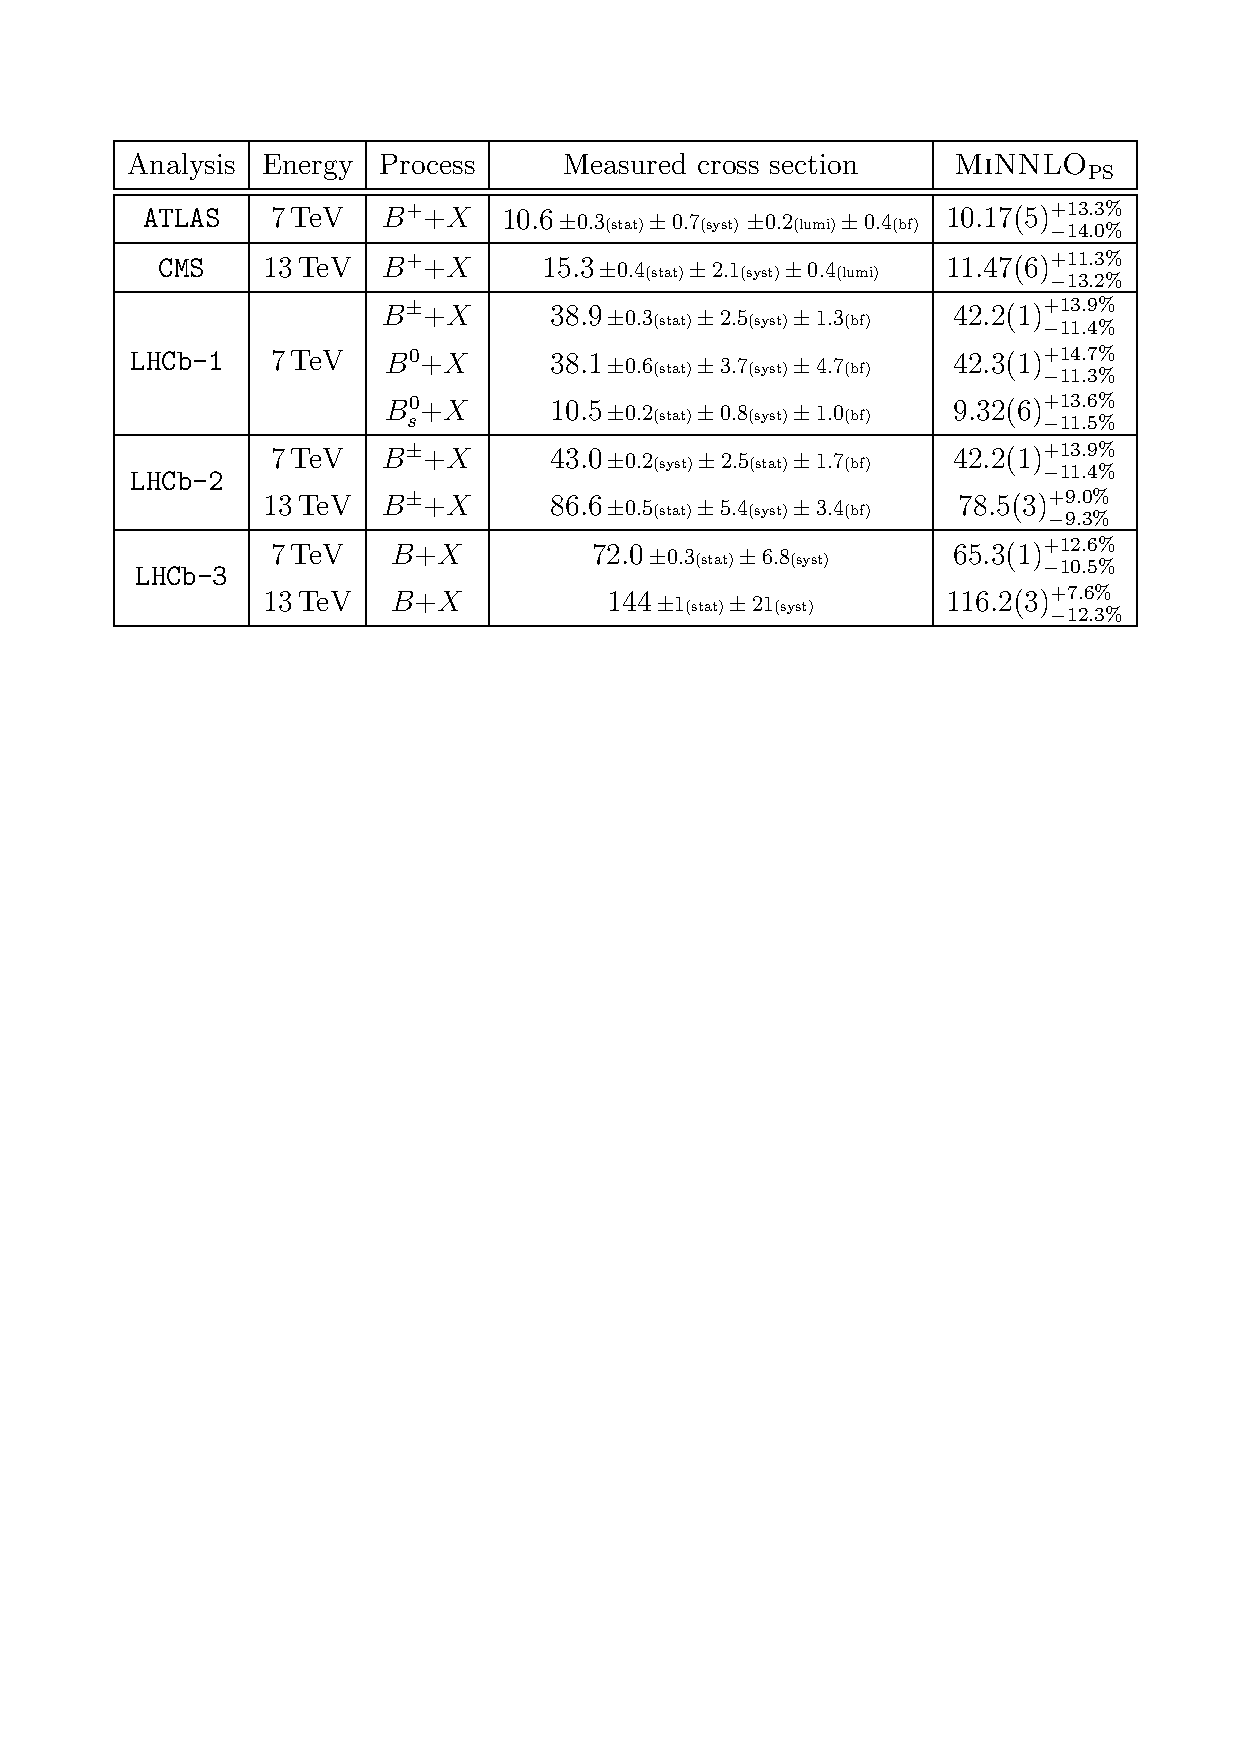
\includegraphics[width=1\linewidth]{plots/bb_table.pdf}
\caption{$B$-hadron cross sections in $\mu$b.}
\label{tab:bb}
\end{center}
\end{table}

The $b\bar b$ \minnlo{}  generator has been developed in \citere{Ratti:} and employed for 
realistic predictions of $B$-hadron production in comparison to various LHC measurements.
By and large, a remarkable description of the measured cross sections is achieved, 
see \tab{tab:bb} for instance. We are currently finalizing a second study where we 
consider $b$-jet observables using our $b\bar b$ \minnlo{} simulation as
well as massless (and massive) NLO+PS dijet simulations. In this context, 
algorithms to appropriately define the bottom flavour in jets play a crucial role, see
\citere{Rhorryspaper} for instance, and we find that the by far dominant effect 
of the difference with to the standard $b$-tagging algorithms used by the experiments
stems from the treatment of $g\to b\bar b$ splittings.
A preliminary comparison of our \minnlo{} predictions against ATLAS data is given in 
\fig{fig:bb}.

\begin{figure}[t]
\begin{center}
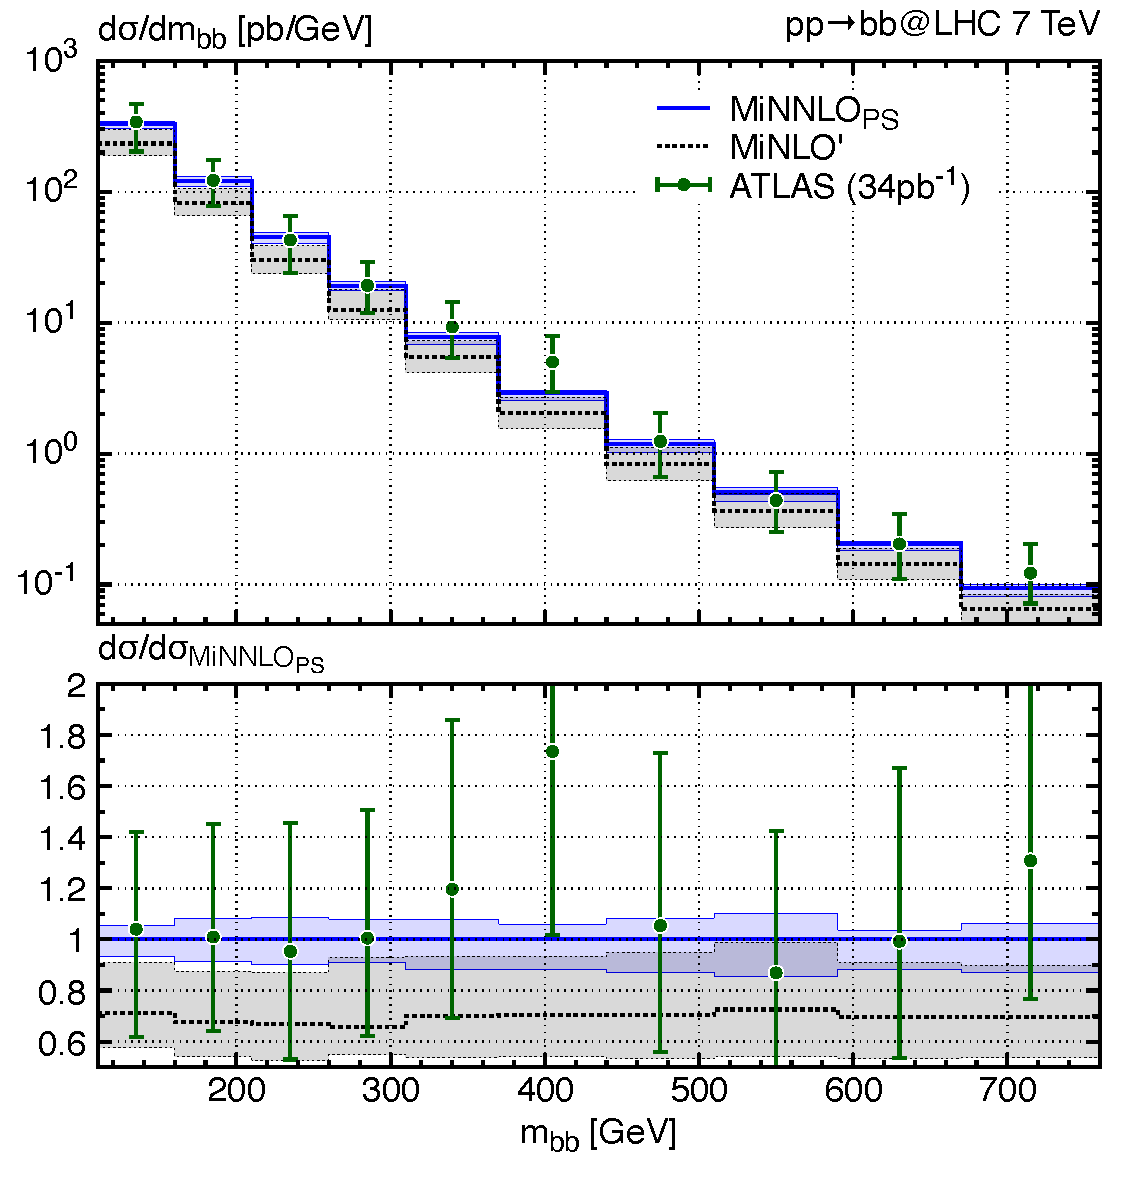
\includegraphics[width=0.95\linewidth]{plots/bjet_mbb.pdf}
\caption{Invariant-mass distribution of leading $b$-jets for \minnlo{} (blue), \minlo{} (grey).}
\label{fig:bb}
\end{center}
\end{figure}
%
\subsubsection[$D$-meson processes at NNLO+PS and prompt neutrino background]{\boldmath{$D$}-meson processes at NNLO+PS \mbox{and prompt neutrino background}}
\begin{Namen}
R. Gauld, T. Giani, A. Mahr, A. Ratti, M. Wiesemann, G. Zanderighi
\end{Namen}

Another important application of the developed \minnlo{} methology is the production
of a charm-quark pair ($c\bar c$) 
in hadron--hadron collisions. While this process also receives
substantial attention by the current LHC experiments, additionally it plays a crucial role in 
the envisaged forward-physics experiments, in particular FASER. Even more crucially,
it is source of a major background to neutrino telescopes, such as ICECUBE, namely
the atmospheric prompt neutrino flux.
In all cases, the underlying mechanism is to produce charm quarks through the collision
of hadrons (either in a controlled collider environment or through cosmic rays interactions 
with the atmosphere), and the charm quarks then hadronize to $D$-mesons. Finally, in 
their further decay process highly energetic neutrinos are produced.

We have implemented a \minnlo{} generator for $c\bar c$ production to compute
$D$-meson cross sections at NNLO+PS. Moreover, we have started to study 
the propagation of particles through the the atmosphere through cascade equation
based on the code Matrix Cascade Equations (MCEq) \cite{} to compute the prompt
atmospheric neutrino flux. In \fig{fig:neutrinoflux} the prompt atmospheric neutrino
flux is shown as a function of the neutrino energy comparing our LO and NLO+PS
inputs to the default MCEq results. As can be seen, the NLO corrections are substantial.
Moreover, the perturbative scale uncertainties (not shown here) are similarly large, 
jeopardizing the precision of the predictions for the neutrino flux. 
This is a severe limitation, which calls for the inclusion of higher-order corrections.
By upgrading these predictions with NNLO accuracy for $c\bar c$ production of 
our \minnlo{} generator we hope to significantly improve the estimation of the 
prompt atmospheric neutrino background in ICECUBE in terms of both accuracy and
precision.

%\begin{figure}[h]
%\begin{center}
%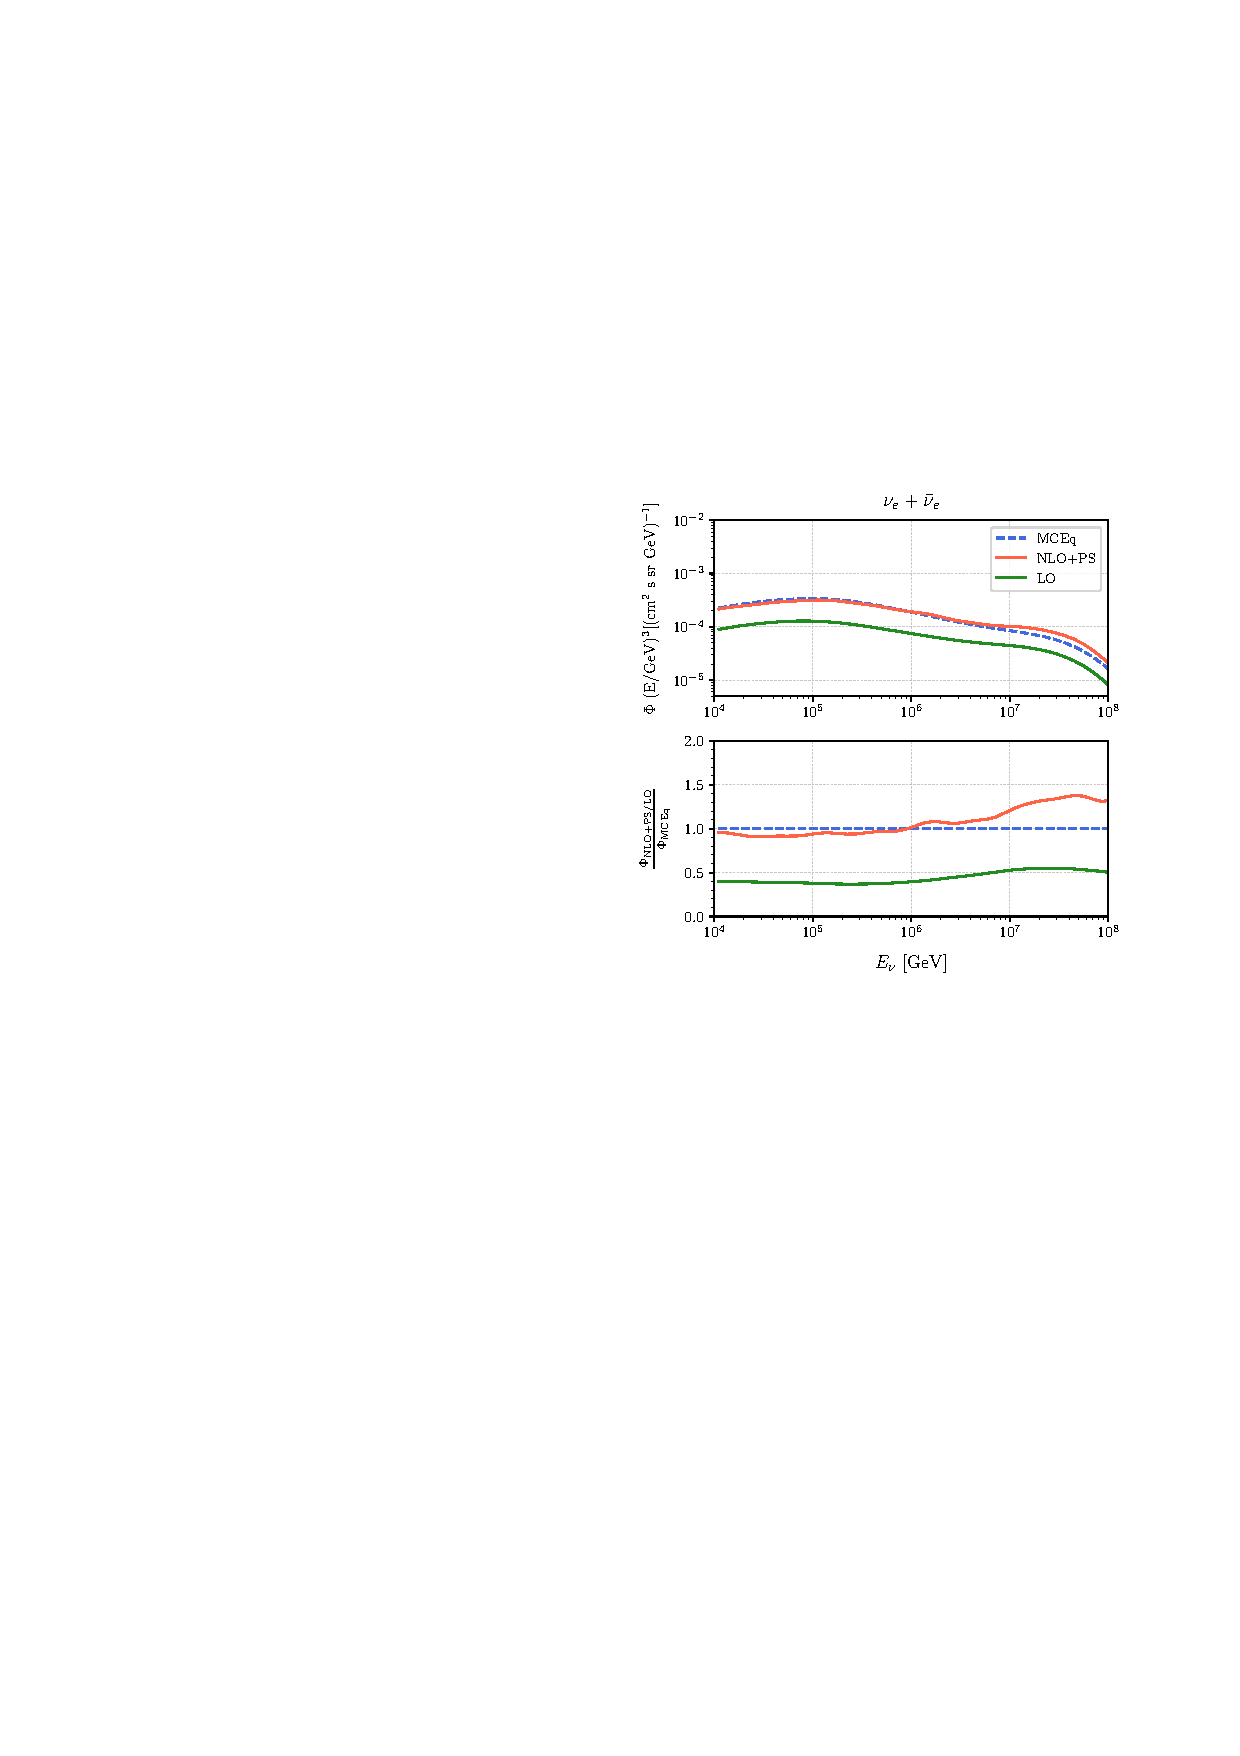
\includegraphics[width=0.95\linewidth]{plots/cc_neutrino_flux}
%\caption{Invariant-mass distribution of leading $b$-jets for \minnlo{} (blue), \minlo{} (grey).}
%\label{fig:neutrinoflux}
%\end{center}
%\end{figure}

%
\subsubsection[\minnlo{} method for heavy-quark plus colour-singlet production and application to $b\bar{b}Z$ process]{\minnlo{} method for heavy-quark plus colour-singlet production and the \boldmath{$b\bar{b}Z$} process}
\begin{Namen}
M. Wiesemann
\end{Namen}
%
{\color{red} ==================\\ ====\; TO BE DONE\; ====\\ ==================}
%
\subsubsection{Associated Higgs production with bottom quarks: a flavour-scheme study at NNLO+PS}
\begin{Namen}
C. Biello, R. Gauld, A. Sankar, M. Wiesemann, G. Zanderighi
\end{Namen}
Higgs production associated with bottom quarks (\bbH{}) is a rare production mode at the LHC, serving as an irreducible background in Higgs-pair searches and gaining potential enhancement in BSM scenarios. Precise predictions of this process are important not only for experimental comparisons but also as a theoretical laboratory for studying heavy-quark effects. In processes involving bottom quarks, predictions can be obtained using different approaches to mass effects. In the scheme with five massless flavours (5FS), the bottom-quark component of the proton is perturbatively generated, enabling the resummation of large logarithmic contributions in the bottom mass. This approach treats the bottom quark as a massless parton, allowing for efficient high-order calculations. In~\citere{Biello:2024vdh}, we presented the first NNLO+PS simulation of this process within the massless scheme. For a more detailed description of bottom-quark kinematics, an alternative approach considers the production of massive bottom quarks in the hard scattering process, along with the Higgs boson, with four massless flavours (4FS). While computationally more demanding, this approach retains all mass effects order by order in perturbative QCD. Working in the \minnlo{} framework, which enables NNLO-accurate predictions for heavy-quark pair production in generic kinematics, we accessed the NNLO corrections in the massive scheme and matched them with a parton shower simulation~\cite{Biello:2024pgo}. Strong tensions between the massless and massive schemes in \bbH{} were observed in the past at lower accuracy, whereas a better agreement is found between the two NNLO+PS predictions, as shown in~\fig{phenofig:bbH}. The two schemes capture complementary aspects of bottom-quark dynamics. A generalised mass-variable flavour number scheme is desirable to achieve precise predictions across the full phase space. Using the method developed in~\citere{Gauld:2021zmq}, we are investigating the isolation of mass power corrections within the massive scheme, aiming to incorporate them into the massless prediction. This would allow us to retain the logarithmic resummation benefits of the massless scheme while systematically accounting for missing power corrections.

\begin{figure}[phtb]
\begin{center}
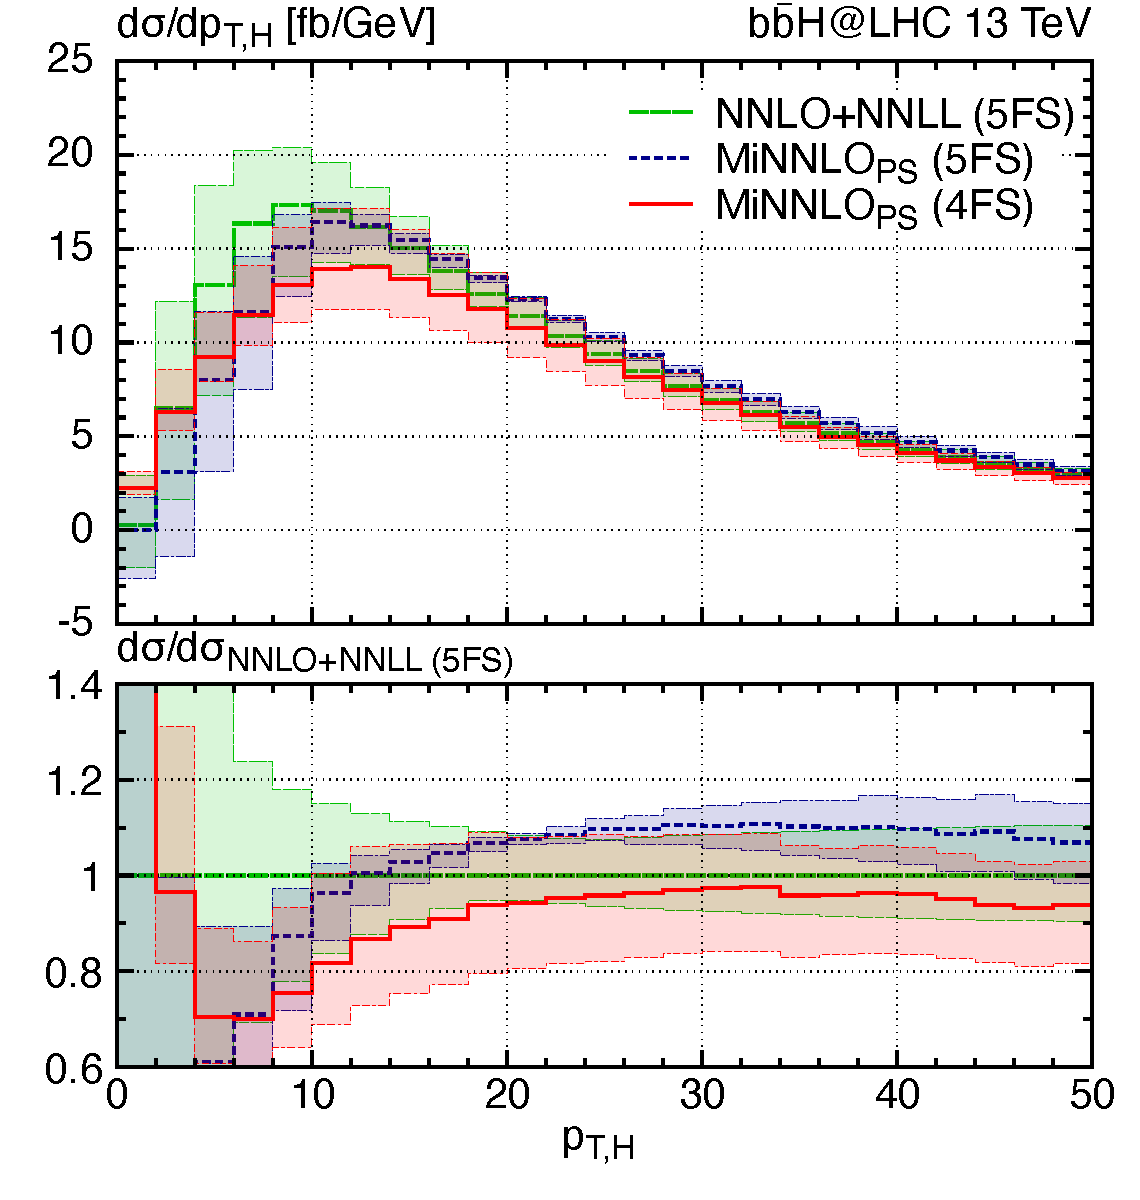
\includegraphics[width=0.95\linewidth]{plots/bbH__ptHspectrum.pdf}
\caption{Transverse spectrum of the Higgs boson produced via the bottom-quark Yukawa interaction at NNLO+PS in the massless (5FS, blue, dotted) and massive (4FS, red, solid) schemes~\cite{Biello:2024pgo}, with an NNLL+NNLO resummation result in the massless scheme (green, dashed).}
\label{phenofig:bbH}
\end{center}
\end{figure}
%
\subsubsection{Off-shell top-quark pair production at NNLO+PS}
\begin{Namen}
C. Biello, C. Signorile-Signorile, M. Wiesemann, G. Zanderighi
\end{Namen}
Given the experimental possibilities provided by the LHC to study the properties of the top quark through decay products, theoretical efforts are required to accurately describe off-shell effects in top-quark pair production. The current advancement of the \minnlo{} method enables the precise simulation of this process, including decay effects in the fully leptonic channel ($pp\rightarrow e^-\bar{\nu}_e\mu^+\nu_\mu b\bar b$). With six particles in the final state at leading order, this represents the highest multiplicity configuration we are currently investigating at NNLO+PS. Its complexity poses both computational and conceptual challenges: we address the high computational cost by improving the numerical efficiency of the code, while in the absence of an exact two-loop amplitude we investigate the development of reliable approximations.
% 
\subsubsection[\minnlo{} method for jet processes using $N$-jettiness]{\minnlo{} method for jet processes using \boldmath{$N$}-jettiness}
\begin{Namen}
M. Ebert, M. Wiesemann, G. Zanderighi, S. Zanoli
\end{Namen}
Despite processes involving light jets in the final state building a 
central class of LHC reactions, no NNLO+PS generators exist for any of them.
With the work of \citere{}, we initiated the further extension of the \minnlo{} method by
formulating it in terms of the $N$-jettiness variable. This jet-resolution variable,
in principle, enables the treatment of any $N\ge 0$ jets in the final state within the 
NNLO+PS matching. In \citere{} we considered the case $N=0$, namely colour-singlet
production, and compared our new $0$-jettiness predictions with the original \minnlo{}
ones using the transverse momentum of the colour singlet.
Moreover, we discussed the $N=1$ case, applicable to colour singlet
plus jet production, by deriving the \minnlo{} formalism for $1$-jettiness.
%
\subsubsection{Inclusion of electroweak corrections in \minnlo{}}
\begin{Namen}
G. Pelliccioli, M. Wiesemann, G. Zanderighi, S. Zanoli
\end{Namen}

\begin{figure}[b!]
\begin{center}
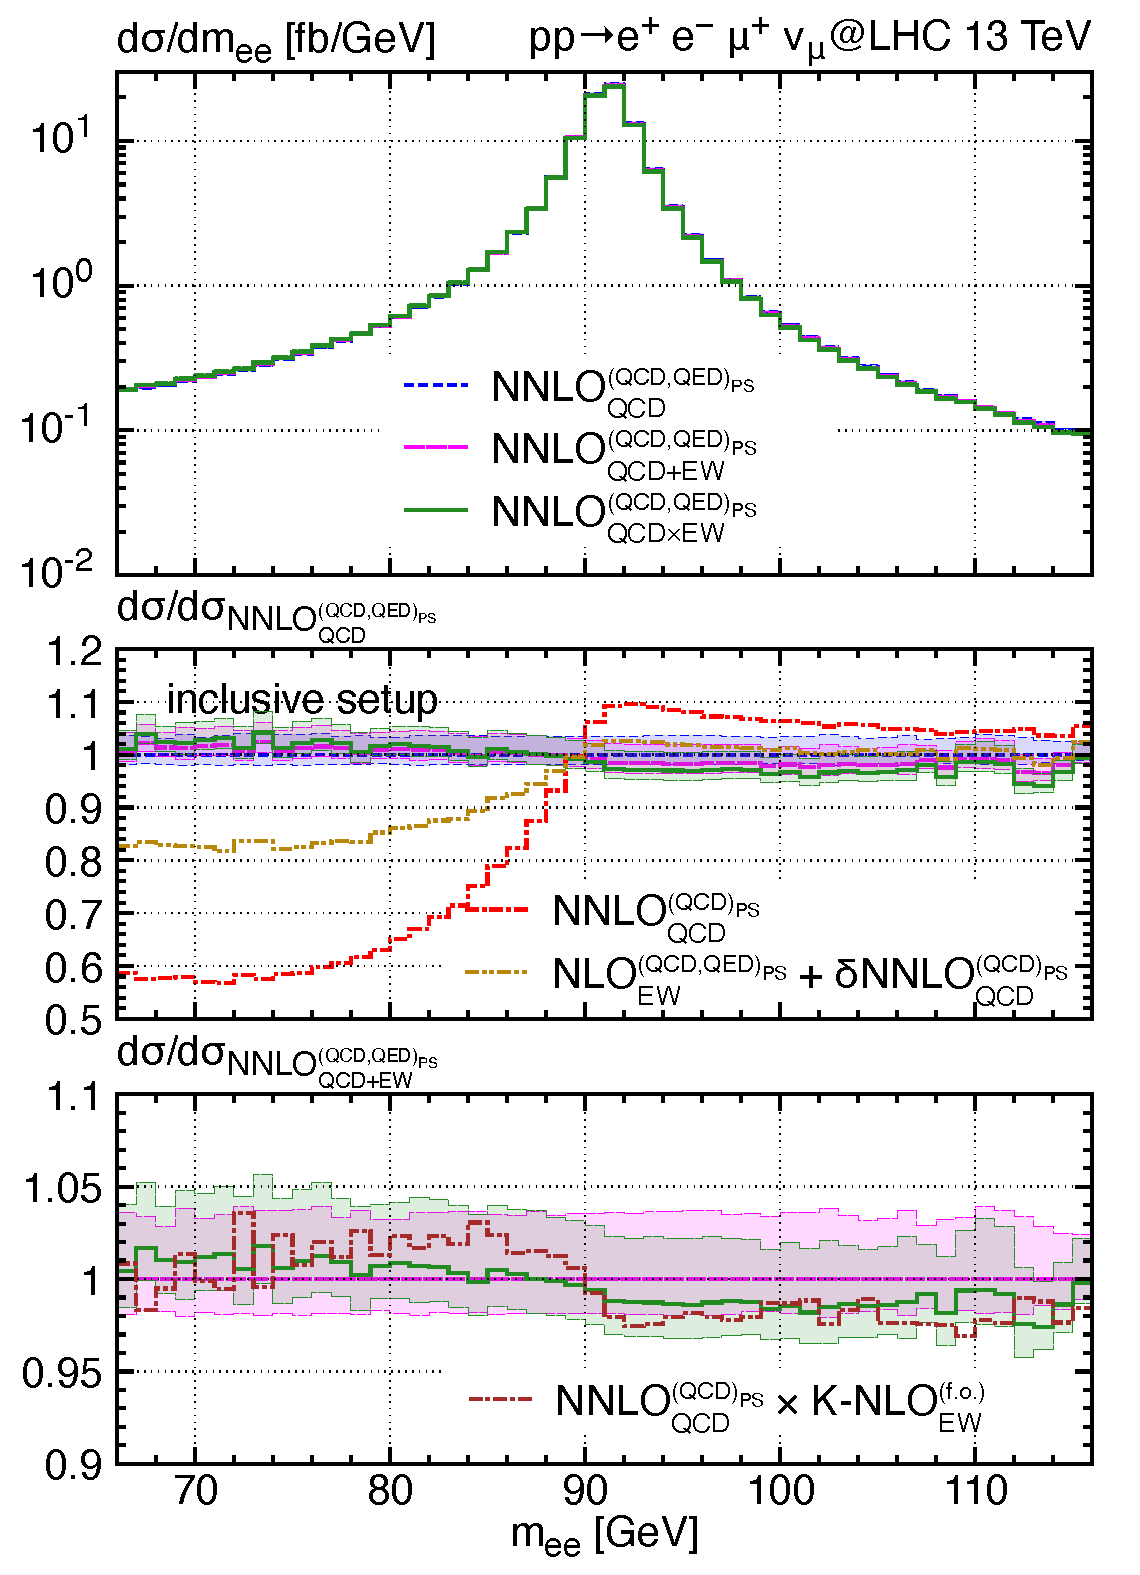
\includegraphics[width=0.95\linewidth]{plots/MiNNLO_EW_WZ_mZ.pdf}
\caption{Dilepton mass in $WZ$ process.}
\label{fig:WZ}
\end{center}
\end{figure}

Although, by and large, 
QCD perturbation theory provides the dominant corrections at hadron 
colliders due to the size of the strong coupling at the relevant energies, 
electroweak (EW) effects are indispensable for the precision programme of the LHC.
In certain phase-space regions EW corrections can even be dominant. This is the case
when obsevables become sensitive to photon radiation, e.g. for invariant-mass 
distribution of a group of leptons, or in the high-energy tails of kinematical distributions,
where EW Sudakov logarithms yield substantial effects.

Given that \minnlo{} provides the most accurate event simulations in 
perturbative QCD to date, the inclusion of EW effects in these predictions
is an important extension. In \citere{}, we developed a \minnlo{} NNLO+PS generator 
as well as a POWHEG NLO+PS  generator including QCD and EW corrections 
for $WZ$ production. We then studied, different approaches to combine the
QCD NNLO+PS predictions with the EW NLO+PS predictions using additive 
and multiplicative matching schemes as well as different treatments of the 
QCD and QED radiation in the parton showers.
As an example, \fig{fig:WZ} shows the crucial importance of photon radiation
to describe the Z-boson line shape (cf. difference with 
red dash-dotted line in first ratio inset, which is the pure QCD prediction).

Currently, we are working on a more sophisticated inclusion of EW effects 
by accounting for NLO EW corrections for $WZ+jet$ production
directly within the \minnlo{} formulae. We then supplement the all-order treatment 
with QED effects to reach NLO EW also for inclusive $WZ$ observables without
extra jets. This approach is currently developed and tested for the Drell-Yan process.


\subsubsection{Polarized NLO+PS predictions and quantum info}
\begin{Namen}
G. Pelliccioli, G. Zanderighi
\end{Namen}
%
{\color{red} ==================\\ ====\; TO BE DONE\; ====\\ ==================}
%
\printbibliography[heading=subbibliography]
\end{refsection}

\subsection{Fixed-order predictions for the hadron--hadron collisions}
%%%%%%%%%%%%%%%%%%%%%%%%%%%%%%%%%%%%%%%%%%%%%%%%%%%%%%%%%%%%%%%%%%%%%%
\begin{refsection}
Section for predictions at hadron-hadron colliders at fixed order.

%
{\color{red} ==================\\ ====\; TO BE DONE\; ====\\ ==================}
%
\subsubsection{Top-mass renormalization in ttbar @ NNLO}
\begin{Namen}
J. Mazzitelli
\end{Namen}
%
{\color{red} ==================\\ ====\; TO BE DONE\; ====\\ ==================}
%
\subsubsection{Wbb @ NNLO}
\begin{Namen}
J. Mazzitelli
\end{Namen}
%
{\color{red} ==================\\ ====\; TO BE DONE\; ====\\ ==================}
%
\subsubsection{Z+c-jet NNLO QCD}
\begin{Namen}
R. Gauld
\end{Namen}
%
{\color{red} ==================\\ ====\; TO BE DONE\; ====\\ ==================}
%
\subsubsection{Off-shell NLO predictions in tt(+X) processes}
\begin{Namen}
G. Pelliccioli
\end{Namen}
%
{\color{red} ==================\\ ====\; TO BE DONE\; ====\\ ==================}
%
\printbibliography[heading=subbibliography]
\end{refsection}


%%%%%%%%%%%%%%%%%%%%%%%%%%%%%%%%%%%%%%%%%%%%%%%%%%%%%%%%%%%%%%%%%%%%%%
\subsection{Precision Higgs physics at the Large Hadron Collider}
%%%%%%%%%%%%%%%%%%%%%%%%%%%%%%%%%%%%%%%%%%%%%%%%%%%%%%%%%%%%%%%%%%%%%%
\begin{refsection}
With the discovery of the Higgs boson in 2012, CERN's Large Hadron Collider has made a 
historic contribution to particle physics. One of the major goals of the physics programme
of the LHC since its discovery is the precise determination of the properties of the Higgs
particles, including its mass and spin, its couplings to other particles, production and decay
rates. To this end, higher-order computations of Higgs reactions at the LHC are indispensable
to reach the most accurate determination of these quantities.

Within our group we have been pushing the precision of Higgs-boson production and decay
processes, at the level of both fixed-order calculations and fully exclusive event simulations,
since many years. 

\subsubsection{Quark-mass effects in Higgs production at NNLO}
\begin{Namen}
M. Niggetiedt
\end{Namen}
%
{\color{red} ==================\\ ====\; TO BE DONE\; ====\\ ==================}
%
\subsubsection{Full top-mass dependence in Higgs production at NNLO+PS}
\begin{Namen}
M. Niggetiedt, M. Wiesemann
\end{Namen}

\begin{figure}[h!]
\begin{center}
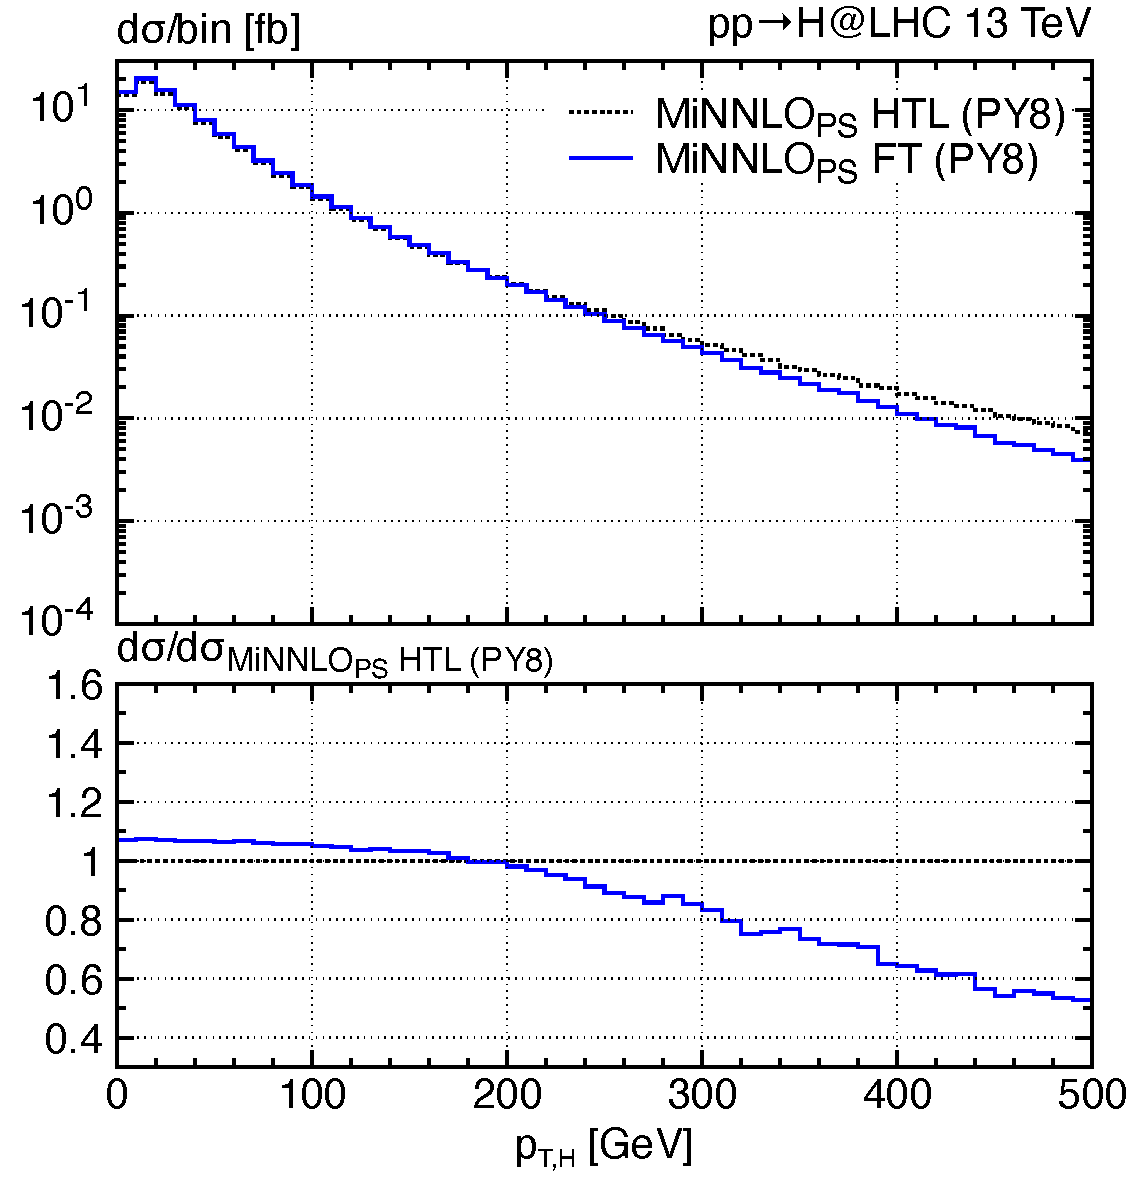
\includegraphics[width=0.95\linewidth]{plots/ptH_diphotons_mass_effect.pdf}
\caption{Top-mass effect in Higgs $p_T$ spectrum.}
\label{fig:topmass_Higgs_pT}
\end{center}
\end{figure}
%
Based on the calculation of the inclusive NNLO cross section in the full theory
including the complete top-mass effects,
we have developed the first (and so far only) 
NNLO+PS generator for the loop-induced 
Higgs production process in gluon fusion in the full theory using 
the \minnlo{} method in \citere{}. Figure\,\ref{fig:topmass_Higgs_pT} shows
the crucial importance of top-mass effect in differential Higgs production
at NNLO+PS at the example of the Higgs transverse-momentum ($p_T$)
spectrum by comparing the full theory result (blue solid) against
the approximation of an infinitely heavy top quark (black, dashed).

In \citere{} we have also quantified the high quality of relevant approximations 
of the top-mass effects at NNLO, which were feasible before, in comparison to our 
novel full-theory results. These results will be useful to provide well-motivated 
approximations of top-mass effects beyond NNLO. Currently, we are extending 
our \minnlo{} calculation by the complete dependence on light-quark mass 
effects (bottom and charm) up to NNLO.
%
\subsubsection{Next-to-soft threshold in \bbH{}}
\begin{Namen}
A. Sankar
\end{Namen}
%
{\color{red} ==================\\ ====\; TO BE DONE\; ====\\ ==================}
%
\subsubsection{Rapidity distribution of pseudoscalar Higgs}
\begin{Namen}
A. Sankar
\end{Namen}
%
{\color{red} ==================\\ ====\; TO BE DONE\; ====\\ ==================}
%
\subsubsection{VBF $H\rightarrow b\bar{b}$ production}
\begin{Namen}
A. Behring, G. Zanderighi
\end{Namen}
%
{\color{red} ==================\\ ====\; TO BE DONE\; ====\\ ==================}
%
\subsubsection{Di-Higgs production at NNLO+PS}
\begin{Namen}
F. Garosi, S. Kumar, M. Wiesemann, G. Zanderighi
\end{Namen}

Our best opportunity to access the Higgs potential at the LHC is through the measurement
of a pair of Higgs bosons. Di-Higgs production is directly sensitive to the trilinear Higgs coupling,
allowing us to put bounds on its value and possibly even measuring its size with the full HL-LHC data.

Since di-Higgs production is a loop-induced $2\to 2$ process the computation of higher-order 
corrections is quite cumbersome, and so far limited to NLO in the full theory. However, by combining
the full-theory NLO predictions with calculations in the heavy-top limit, it is possible to obtain 
meaningful approximations of the NNLO cross section. Following this idea, we are currently 
implementing a new NNLO+PS generator for Higgs-pair production using the \minnlo{} method.


\printbibliography[heading=subbibliography]
\end{refsection}

%%%%%%%%%%%%%%%%%%%%%%%%%%%%%%%%%%%%%%%%%%%%%%%%%%%%%%%%%%%%%%%%%%%%%%
\subsection{Tools and methods for higher-order predictions}
%%%%%%%%%%%%%%%%%%%%%%%%%%%%%%%%%%%%%%%%%%%%%%%%%%%%%%%%%%%%%%%%%%%%%%
\begin{refsection}
Space for a nice introduction.

%
{\color{red} ==================\\ ====\; TO BE DONE\; ====\\ ==================}
%
\subsubsection{LASS: a subtraction scheme method at NNLO}
\begin{Namen}
G. Pelliccioli, A. Ratti, C. Signorile-Signorile
\end{Namen}
Include formulation and Strongly-ordered infrared counterterms from factorisation.

%
{\color{red} ==================\\ ====\; TO BE DONE\; ====\\ ==================}
%
\subsubsection{New formulation of Nested Soft-Collinear Subtraction Scheme}
\begin{Namen}
C. Signorile-Signorile
\end{Namen}
%
{\color{red} ==================\\ ====\; TO BE DONE\; ====\\ ==================}
%
\subsubsection{Four-loop renormalisation of pseudoscalar operators}
\begin{Namen}
M. Niggetiedt
\end{Namen}
%
{\color{red} ==================\\ ====\; TO BE DONE\; ====\\ ==================}
%
\subsubsection{Soft function at N3LO}
\begin{Namen}
M. Delto, C. Wang
\end{Namen}
%
{\color{red} ==================\\ ====\; TO BE DONE\; ====\\ ==================}
%
\subsubsection{Reclassifying Feynman Integrals as Special Functions}
\begin{Namen}
C. Wang
\end{Namen}
%
{\color{red} ==================\\ ====\; TO BE DONE\; ====\\ ==================}
%
\printbibliography[heading=subbibliography]
\end{refsection}

%%%%%%%%%%%%%%%%%%%%%%%%%%%%%%%%%%%%%%%%%%%%%%%%%%%%%%%%%%%%%%%%%%%%%%
\subsection{\mbox{Beyond hadron--hadron colliders}}
%%%%%%%%%%%%%%%%%%%%%%%%%%%%%%%%%%%%%%%%%%%%%%%%%%%%%%%%%%%%%%%%%%%%%%
\begin{refsection}
The application and development of new computational methods and simulation tools has also 
been pursued for different collider environments, such as those from lepton--hadron or lepton--lepton collisions.
%
Scattering processes with an initial-state lepton or leptons introduce different theoretical 
challenges as compared to that of hadron--hadron collisions, but, at the same time, tools
and methods developed during the LHC era can be adapted to leptonic initial states
in many cases, where the state of research is often still at the level of 20 years ago or more.

Moreover, lepton collisions offer exciting opportunities to study the properties of the strong force, QED interactions, and even Higgs properties in a relatively clean environment.
%
Such developments allow to re-visit the available data from colliders such as HERA and LEP with more precise theoretical simulations and inputs, increase the precision of simulation tools available for active experiments (e.g. IceCube and KM3NeT), and also provide a new level of theoretical precision for future experiments such as the EIC or a potential high-energy $e^+e^-$ collider. 
%
\subsubsection{NNLO+PS prediction for di-jet production at lepton colliders}
\begin{Namen}
F. Koenig, R. Schorer, M. Wiesemann, G. Zanderighi
\end{Namen}
%
{\color{red} ==================\\ ====\; TO BE DONE\; ====\\ ==================}
%
\subsubsection{NLO+PS predictions for charged-lepton and neutrino induced DIS}
\begin{Namen}
R. Gauld, G. Zanderighi
\end{Namen}
The POWHEG method of matching fixed-order predictions with parton showers at NLO in QCD has been successfully applied to hadron-hadron collisions for a vast range of processes. As a consequence of the genuinely different kinematics encountered in lepton-hadron collisions, substantial extensions to the POWHEX BOX framework had to be undertaken to enable this method to be applied in this new collision environment~\cite{Banfi:2023mhz}.
The same extensions have also enabled the method to be applied in the case of neutrino-induced collisions~\cite{FerrarioRavasio:2024kem}, which now allow for the fully exclusive simulation of (ultra) high-energy neutrino-nucleon collisions.
These new (publicly available) tools improve the precision of fully exclusive simulations of lepton-hadron collisions. This has direct implications for past experiments such as HERA, ongoing measurements at forward detectors at the LHC (e.g. Faser$\nu$, FPF) and large volume neutrino experiments (IceCube, KM3NeT, Baikal), as well as forthcoming colliders such as the EIC and proposed next-generation neutrino detectors.
%
\subsubsection{Strong-coupling constant determination}
\begin{Namen}
P. Nason, G. Zanderighi
\end{Namen}
%
Theoretical predictions for collider processes heavily rely on
perturbative QCD calculations, which in turn require as input the
value of the strong coupling constant $\alpha_s$. The uncertainty on
$\alpha_s$ is in several cases the limiting factor in providing more
accurate perturbative predictions which can then be comapred to
precise data from Run III of the LHC and the foreseen High Luminosity
upgrade.
%
G.~Zanderighi has been driving and steering progress in reducing this
uncertainty on three distinct fronts.

First, she is the theory editor of the section Quantum Chromodynamics
(QCD) of the Review of the Particle Data Group
(PDG)~\cite{ParticleDataGroup:2022pth,ParticleDataGroup:2024cfk},
which besides providing a summary of the state of the art of QCD
calculations and comparisons to data, presents an update, very two
years, the world average of the strong coupling $\alpha_s$. This
``world'' avarage is taken as reference input in all QCD
calculation. A decision on which extraciton to include and how to
compbine them is therefore assessed with greatest care.

Furthermore, G. Zanderighi has been studying more in detail the
discrepancy in the determination of $\alpha_s$ from event shapes,
where different determinations based on analytic models or Monte Carlo
estimates of the non-perturbative corrections lead to barely
consistent results.

Recent work of G. Zanderighi~\cite{Nason:2025qbx} is an extension of a previous
publication~\cite{Nason:2023asn} where we fitted the strong coupling
$\alpha_s$ together with the non-perturbative parameter $\alpha_0$ from
event-shape and jet-shape distributions using power corrections
computed for the first time in the three-jet region.
%
In ref.~\cite{Nason:2023asn} only ALEPH data at the $Z$-pole were
used in the fit. Ref., instead, we include a large data sample from
various $e^+e^-$ experiments at energies ranging from 22 to 207
GeV and revisited the treatment of theoretical uncertainties.
%
In Ref.~\cite{Nason:2025qbx} it is shown that the inclusion of different
energies, while not changing the central fit result considerably,
helps to disentangle the dependence of perturbative and
non-perturbative corrections.
%
The best fit result is $\alpha_s(M_Z) = 0.1181 \substack{ +0.0002
  \\ -0.0005} \substack{ +0.0018 \\ -0.0021}$, where the first error
includes experimental uncertianties and the second one includes
uncertainties associated with scale variation, mass effects, fit
limits, non-perturbative schemes and non-perturbative uncertainties.
  %




\subsubsection{Time-like matching conditions at the threshold}
\begin{Namen}
C. Biello
\end{Namen}
Threshold conditions are matching ingredients in the DGLAP evolution within the Variable Flavour Number Scheme, governing the effects of crossing a heavy-quark threshold. They represent the final missing process-independent component needed for the NNLO extraction of Fragmentation Functions (FFs), which are time-like non-perturbative objects enabling predictions for identified hadrons. In~\citere{Biello:2024zti}, we have extended the formalism along the lines of~\citere{Cacciari:2005ry} for deriving the matching conditions at NNLO QCD, employing matrix elements from electron-positron annihilation. At this perturbative order, light-quark to hadron FFs require a threshold correction, which we have analytically computed. Future studies will focus on completing the set by deriving threshold conditions for the fragmentation of a gluon or a heavy quark. These investigations are useful not only for achieving formal accuracy in FF fits but also for obtaining deeper insights into the fundamental structure of hadrons. In this context, the known NNLO space-like threshold conditions have been used in providing evidence for intrinsic charm in the proton. These studies showed a non-vanishing charm-flavour wave-function component that is not perturbatively generated by DGLAP evolution to LHC energies, given the threshold conditions at the heavy-quark mass~\cite{Ball:2022qks}.
%
\subsubsection{Mass power corrections for fragmentation functions}
\begin{Namen}
F. Ahmadova, R. Gauld
\end{Namen}
The theoretical description for scattering processes in which a heavy-flavour hadron is identified are typically based on either a massive or a massless description of the quark fragmentation process. These approaches are applicable at either low- or high-energy scales, and for very simple cases a combination of these methods are possible.
On-going work in the group also aims to establish a fully differential description of identified hadron production in a general mass variable flavour number scheme. These developments allow for unified description of identified hadron production in complicated scattering processes with jets and identified hadrons.
These advancements will have important implications for LHC measurements involving heavy-flavour jets, where the standard experimental approach of flavour tagging use the kinematics of identified heavy-flavour hadrons to establish the flavour quantum numbers of jets.
%
\subsubsection{Tetraquarks}
\begin{Namen}
C. Wang
\end{Namen}
%
{\color{red} ==================\\ ====\; TO BE DONE\; ====\\ ==================}
%
\subsubsection{Neutrino content of the muon}
\begin{Namen}
F. Garosi
\end{Namen}
%
{\color{red} ==================\\ ====\; TO BE DONE\; ====\\ ==================}
%
\printbibliography[heading=subbibliography]
\end{refsection}

%%%%%%%%%%%%%%%%%%%%%%%%%%%%%%%%%%%%%%%%%%%%%%%%%%%%%%%%%%%%%%%%%%%%%%
\subsection{Beyond Standard Model seaches}
%%%%%%%%%%%%%%%%%%%%%%%%%%%%%%%%%%%%%%%%%%%%%%%%%%%%%%%%%%%%%%%%%%%%%%
\begin{refsection}
Searches for physics beyond the Standard Model (BSM) physics remain a major goal of collider physics experiments.
The sensitivity of many of the conducted searches rely on the availability of precise simulations of signal and background processes, in particular those aiming to observe indirect signals of BSM in terms of (small) deviations of known SM processes or signals of missing energy. 
The development of such tools are essential for the interpretation of collider data, but can also play a crucial role in the design of future experiments~\cite{Bechtle:2024atq}.
%
\subsubsection{Bringing precision to SMEFT}
\begin{Namen}
R. Gauld, M. Niggetiedt%, L. Schnell, U. Haisch, J. Weiss
\end{Namen}
The SM effective field theory (SMEFT) offers a model-independent framework to indirectly search for (non-resonant) signals of BSM.
The potential interpretation of data in this framework is facilitated by the availability of high precision calculations in SMEFT.
To this end, and building upon the expertise developed for predictions within the SM, several high precision studies and calculations relevant for selected Electroweak and Higgs production processes at the LHC have been performed.
These include the development of a NNLO+PS generator for the description of the process $pp\to Vh$~\cite{Gauld:2023gtb}, the interpretation of high-energy LHC data for the $pp\to Zj$ process~\cite{Gauld:2024glt}, as well as the calculation of two-loop amplitudes for Higgs production in the presence of a modified cubic Higgs self-coupling~\cite{Haisch:2024nzv}.
These studies have been performed in collaboration with members of the independent research group of U. Haisch, and we refer the reader to that Section for more details on these projects.
%
\subsubsection{Polarised NLO+PS predictions in SMEFT}
\begin{Namen}
J. Linder, G. Pelliccioli, G. Zanderighi
\end{Namen}
%
{\color{red} ==================\\ ====\; TO BE DONE\; ====\\ ==================}
%
\subsubsection{MEM method in Powheg and \minnlo{}}
\begin{Namen}
U. Haisch, J. Linder, M. Wiesemann, G. Zanderighi
\end{Namen}
%
{\color{red} ==================\\ ====\; TO BE DONE\; ====\\ ==================}
%
\subsubsection{New collider proposal for dark matter studies}
\begin{Namen}
R. Gauld
\end{Namen}
The nature of Dark Matter remains an outstanding question in elementary particle physics, with searches only producing negative (or irreproducible) results.
This suggests to conduct experiments which can probe currently unexplored regions of the parameter space of Dark Matter models.
The Lohengrin experiment is an example of such a proposal~\cite{Bechtle:2024atq} which aims to perform the fixed-target missing momentum based technique to search for dark-sector particles (the ~GeV energy electron beam is provided by the ELSA Accelerator in Bonn).
A simulation tool (lohengrin++) has been developed jointly at the MPP (with Uni. Bonn) for the scattering of electrons and nuclear targets for both signals of (light) Dark Matter as well as SM background processes. This tool has already played an important role in the detector design (feasibility study) and will continue to be developed as planning for the experiment continues. An example of a (differential) Signal-to-Background study for a 10~MeV Dark Photon produced in the collision of a 3.2~GeV electron beam incident on Tungsten is shown in Fig.~{X}.
%
\subsubsection{$b\rightarrow s \gamma$ corrections for the physical value of the charm mass}
\begin{Namen}
M. Niggetiedt
\end{Namen}
%
{\color{red} ==================\\ ====\; TO BE DONE\; ====\\ ==================}
%
\subsubsection{Cubic Higgs self interaction in Higgs plus jet at two loops}
\begin{Namen}
U. Haisch, M. Niggetiedt
\end{Namen}
%
{\color{red} ===========================\\ ==\; REMOVE? $\rightarrow$ IN ULI's REPORT\; ==\\ ===========================}
%
\printbibliography[heading=subbibliography]
\end{refsection}


% ----------------------------------------------------------------------
\clearpage
\onecolumn
% ----------------------------------------------------------------------
\end{document}
% ----------------------------------------------------------------------
